\documentclass[11pt,a4paper]{article}
\usepackage[utf8]{inputenc}
\usepackage{amsmath,amssymb,amsthm}
\usepackage{tikz}
\usetikzlibrary{shapes.gates.logic.US,shapes.gates.logic.IEC,calc,positioning,arrows.meta,decorations.pathmorphing}
\usepackage{algorithm}
\usepackage{algpseudocode}
\usepackage{hyperref}
\usepackage[margin=1in]{geometry}

\newtheorem{theorem}{Theorem}
\newtheorem{lemma}[theorem]{Lemma}
\newtheorem{definition}{Definition}
\newtheorem{claim}{Claim}

\title{Reducing Circuit SAT to Maximum Independent Set}
\author{Notes on NP-Completeness Reductions}
\date{}

\begin{document}
\maketitle

\begin{abstract}
This note presents the polynomial-time reduction from Circuit SAT to the Maximum Independent Set (MIS) problem, establishing that MIS is NP-complete. The reduction proceeds in two stages: first from Circuit SAT to 3-SAT via the Tseytin transformation, then from 3-SAT to MIS using clause gadgets. We provide detailed constructions with illustrative TikZ diagrams.
\end{abstract}

\section{Introduction to NP-Completeness}

Computational complexity theory classifies problems by the resources required to solve them. A central concept in this field is \textbf{NP-completeness}, which identifies the ``hardest'' problems in the class NP.

\begin{definition}[The Class P]
P is the class of decision problems solvable by a deterministic Turing machine in polynomial time. These are problems we consider ``efficiently solvable.''
\end{definition}

\begin{definition}[The Class NP]
NP (nondeterministic polynomial time) is the class of decision problems for which a ``yes'' answer can be \emph{verified} in polynomial time, given an appropriate certificate (or witness). Equivalently, NP is the class of problems solvable by a nondeterministic Turing machine in polynomial time.
\end{definition}

\begin{definition}[Polynomial-Time Reduction]
A problem $A$ is \emph{polynomial-time reducible} to problem $B$, written $A \leq_p B$, if there exists a polynomial-time computable function $f$ such that for all instances $x$:
\[
x \in A \iff f(x) \in B
\]
Intuitively, if we can solve $B$ efficiently, then we can solve $A$ efficiently by first transforming the input.
\end{definition}

\begin{definition}[NP-Complete]
A problem $B$ is \textbf{NP-complete} if:
\begin{enumerate}
    \item $B \in \mathrm{NP}$ (solutions can be verified in polynomial time), and
    \item Every problem $A \in \mathrm{NP}$ satisfies $A \leq_p B$ (B is NP-hard).
\end{enumerate}
\end{definition}

NP-complete problems are significant because they represent a class of problems that are all polynomially equivalent---if any one of them admits a polynomial-time algorithm, then \emph{all} problems in NP can be solved in polynomial time (implying P = NP). The famous Cook-Levin theorem established that Circuit SAT (and Boolean SAT) are NP-complete, providing the foundation for proving other problems NP-complete through polynomial-time reductions.

In this note, we demonstrate that the Maximum Independent Set problem is NP-complete by reducing from Circuit SAT, which is known to be NP-complete.

\section{Problem Definitions}

\begin{definition}[Circuit SAT]
Given a Boolean circuit $C$ with $n$ input variables $x_1, \ldots, x_n$ and a single output, determine whether there exists an assignment to the input variables such that $C$ outputs \texttt{TRUE}.
\end{definition}

\begin{definition}[Maximum Independent Set (MIS)]
Given an undirected graph $G = (V, E)$ and an integer $k$, determine whether there exists a subset $S \subseteq V$ with $|S| \geq k$ such that no two vertices in $S$ are adjacent.
\end{definition}

\begin{definition}[3-SAT]
Given a Boolean formula $\phi$ in conjunctive normal form (CNF) where each clause contains exactly three literals, determine whether there exists a satisfying assignment.
\end{definition}

\section{Overview of the Reduction Chain}

The reduction from Circuit SAT to MIS proceeds in two steps:
\[
\text{Circuit-SAT} \leq_p \text{3-SAT} \leq_p \text{Independent Set}
\]

\begin{figure}[h]
\centering
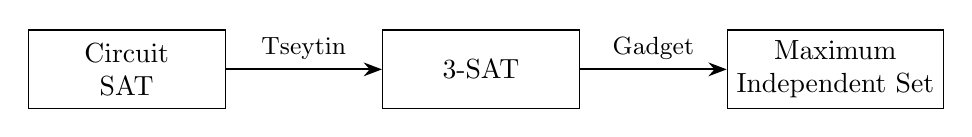
\begin{tikzpicture}[
    box/.style={rectangle, draw, minimum width=2.5cm, minimum height=1cm, align=center},
    arrow/.style={-{Stealth}, thick}
]
    \node[box] (csat) at (0,0) {Circuit\\SAT};
    \node[box] (3sat) at (4.5,0) {3-SAT};
    \node[box] (mis) at (9,0) {Maximum\\Independent Set};

    \draw[arrow] (csat) -- (3sat) node[midway, above] {\small Tseytin};
    \draw[arrow] (3sat) -- (mis) node[midway, above] {\small Gadget};
\end{tikzpicture}
\caption{The reduction chain from Circuit SAT to Maximum Independent Set}
\end{figure}

\section{Step 1: Circuit SAT to 3-SAT (Tseytin Transformation)}

The Tseytin transformation converts a Boolean circuit into an equisatisfiable CNF formula with size linear in the circuit size.

\subsection{Key Idea}

For each gate in the circuit, we introduce a new variable representing its output and add clauses that enforce the gate's behavior. This avoids the exponential blowup that can occur with naive conversion.

\subsection{Gate Encodings}

For each type of gate, we create CNF clauses that are satisfiable if and only if the output correctly represents the gate's function:

\paragraph{AND Gate:} For $C = A \land B$:
\[
(\neg A \lor \neg B \lor C) \land (A \lor \neg C) \land (B \lor \neg C)
\]

\paragraph{OR Gate:} For $C = A \lor B$:
\[
(A \lor B \lor \neg C) \land (\neg A \lor C) \land (\neg B \lor C)
\]

\paragraph{NOT Gate:} For $C = \neg A$:
\[
(\neg A \lor \neg C) \land (A \lor C)
\]

\begin{figure}[h]
\centering
\begin{tikzpicture}[
    circuit logic US,
    every circuit symbol/.style={thick},
    scale=1.2
]
    % AND gate
    \node[and gate US, draw, minimum size=1cm] (and) at (0,0) {};
    \node[left] at (and.input 1) {$A$};
    \node[left] at (and.input 2) {$B$};
    \node[right] at (and.output) {$C$};
    \node[below=0.8cm] at (and.south) {\small $C = A \land B$};

    % OR gate
    \node[or gate US, draw, minimum size=1cm] (or) at (4,0) {};
    \node[left] at (or.input 1) {$A$};
    \node[left] at (or.input 2) {$B$};
    \node[right] at (or.output) {$C$};
    \node[below=0.8cm] at (or.south) {\small $C = A \lor B$};

    % NOT gate
    \node[not gate US, draw, minimum size=0.6cm] (not) at (8,0) {};
    \node[left] at (not.input) {$A$};
    \node[right] at (not.output) {$C$};
    \node[below=0.8cm] at (not.south) {\small $C = \neg A$};
\end{tikzpicture}
\caption{Basic logic gates used in circuits}
\end{figure}

\subsection{Complete Example}

Consider the circuit computing $f(x_1, x_2, x_3) = (x_1 \land x_2) \lor x_3$:

\begin{figure}[h]
\centering
\begin{tikzpicture}[
    circuit logic US,
    every circuit symbol/.style={thick},
    scale=1.0
]
    % Inputs
    \node (x1) at (0, 1) {$x_1$};
    \node (x2) at (0, 0) {$x_2$};
    \node (x3) at (0, -1.5) {$x_3$};

    % AND gate
    \node[and gate US, draw, minimum size=0.8cm] (and) at (2.5, 0.5) {};
    \draw (x1.east) -- ++(0.5,0) |- (and.input 1);
    \draw (x2.east) -- ++(0.5,0) |- (and.input 2);

    % Intermediate variable g1
    \node[above=0.1cm] at (and.output) {\small $g_1$};

    % OR gate
    \node[or gate US, draw, minimum size=0.8cm] (or) at (5.5, -0.25) {};
    \draw (and.output) -- ++(0.5,0) |- (or.input 1);
    \draw (x3.east) -- ++(3.2,0) |- (or.input 2);

    % Output
    \node (out) at (7, -0.25) {$f$};
    \draw (or.output) -- (out);
\end{tikzpicture}
\caption{Circuit for $f(x_1, x_2, x_3) = (x_1 \land x_2) \lor x_3$}
\end{figure}

The Tseytin transformation produces:
\begin{align*}
\phi = \quad & (\neg x_1 \lor \neg x_2 \lor g_1) \land (x_1 \lor \neg g_1) \land (x_2 \lor \neg g_1) && \text{(AND gate)} \\
\land\quad & (g_1 \lor x_3 \lor \neg f) \land (\neg g_1 \lor f) \land (\neg x_3 \lor f) && \text{(OR gate)} \\
\land\quad & (f) && \text{(output must be TRUE)}
\end{align*}

\begin{theorem}
The Tseytin transformation runs in polynomial time and produces a formula $\phi$ such that:
\begin{enumerate}
    \item $|\phi| = O(|C|)$ where $|C|$ is the size of the circuit
    \item The circuit $C$ is satisfiable if and only if $\phi$ is satisfiable
\end{enumerate}
\end{theorem}

\section{Step 2: 3-SAT to Maximum Independent Set}

\subsection{Construction}

Given a 3-SAT formula $\phi$ with $m$ clauses $C_1, \ldots, C_m$, we construct a graph $G_\phi$ and set $k = m$.

\paragraph{Vertex Construction:} For each clause $C_j = (\ell_{j,1} \lor \ell_{j,2} \lor \ell_{j,3})$, create three vertices $v_{j,1}, v_{j,2}, v_{j,3}$, one for each literal.

\paragraph{Edge Construction:} Add two types of edges:
\begin{enumerate}
    \item \textbf{Clause edges (triangles):} For each clause $C_j$, connect all three vertices in a triangle:
    \[
    \{v_{j,1}, v_{j,2}\}, \{v_{j,2}, v_{j,3}\}, \{v_{j,1}, v_{j,3}\}
    \]
    \item \textbf{Conflict edges:} For any two vertices $v_{j,a}$ and $v_{k,b}$ (from different clauses) whose labels are complementary literals (i.e., one is $x_i$ and the other is $\neg x_i$), add an edge.
\end{enumerate}

\begin{figure}[h]
\centering
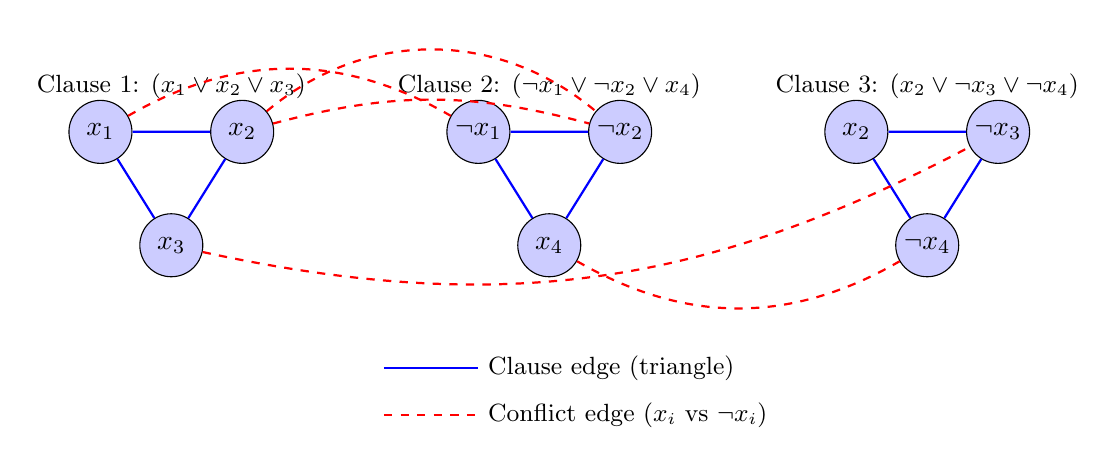
\begin{tikzpicture}[
    vertex/.style={circle, draw, fill=blue!20, minimum size=8mm, inner sep=1pt},
    clause_edge/.style={thick, blue},
    conflict_edge/.style={thick, red, dashed},
    scale=1.2
]
    % Clause 1: (x1 v x2 v x3)
    \node[vertex] (v11) at (0, 2) {$x_1$};
    \node[vertex] (v12) at (1.5, 2) {$x_2$};
    \node[vertex] (v13) at (0.75, 0.8) {$x_3$};

    % Clause 1 triangle
    \draw[clause_edge] (v11) -- (v12);
    \draw[clause_edge] (v12) -- (v13);
    \draw[clause_edge] (v13) -- (v11);

    \node[above=0.3cm] at (0.75, 2) {\small Clause 1: $(x_1 \lor x_2 \lor x_3)$};

    % Clause 2: (not x1 v not x2 v x4)
    \node[vertex] (v21) at (4, 2) {$\neg x_1$};
    \node[vertex] (v22) at (5.5, 2) {$\neg x_2$};
    \node[vertex] (v23) at (4.75, 0.8) {$x_4$};

    % Clause 2 triangle
    \draw[clause_edge] (v21) -- (v22);
    \draw[clause_edge] (v22) -- (v23);
    \draw[clause_edge] (v23) -- (v21);

    \node[above=0.3cm] at (4.75, 2) {\small Clause 2: $(\neg x_1 \lor \neg x_2 \lor x_4)$};

    % Clause 3: (x2 v not x3 v not x4)
    \node[vertex] (v31) at (8, 2) {$x_2$};
    \node[vertex] (v32) at (9.5, 2) {$\neg x_3$};
    \node[vertex] (v33) at (8.75, 0.8) {$\neg x_4$};

    % Clause 3 triangle
    \draw[clause_edge] (v31) -- (v32);
    \draw[clause_edge] (v32) -- (v33);
    \draw[clause_edge] (v33) -- (v31);

    \node[above=0.3cm] at (8.75, 2) {\small Clause 3: $(x_2 \lor \neg x_3 \lor \neg x_4)$};

    % Conflict edges
    \draw[conflict_edge] (v11) to[bend left=30] (v21);
    \draw[conflict_edge] (v12) to[bend left=15] (v22);
    \draw[conflict_edge] (v13) to[bend right=20] (v32);
    \draw[conflict_edge] (v23) to[bend right=30] (v33);
    \draw[conflict_edge] (v12) to[bend left=40] (v22);

    % Legend
    \draw[clause_edge] (3, -0.5) -- (4, -0.5);
    \node[right] at (4, -0.5) {\small Clause edge (triangle)};
    \draw[conflict_edge] (3, -1) -- (4, -1);
    \node[right] at (4, -1) {\small Conflict edge ($x_i$ vs $\neg x_i$)};
\end{tikzpicture}
\caption{Graph construction for the formula $\phi = (x_1 \lor x_2 \lor x_3) \land (\neg x_1 \lor \neg x_2 \lor x_4) \land (x_2 \lor \neg x_3 \lor \neg x_4)$}
\end{figure}

\subsection{Intuition Behind the Construction}

\begin{itemize}
    \item The \textbf{triangle structure} ensures we can select at most one vertex per clause (choosing the ``true'' literal).
    \item The \textbf{conflict edges} ensure we cannot simultaneously select $x_i$ from one clause and $\neg x_i$ from another (consistency).
    \item An independent set of size $m$ corresponds to selecting exactly one true literal per clause without contradictions.
\end{itemize}

\begin{figure}[h]
\centering
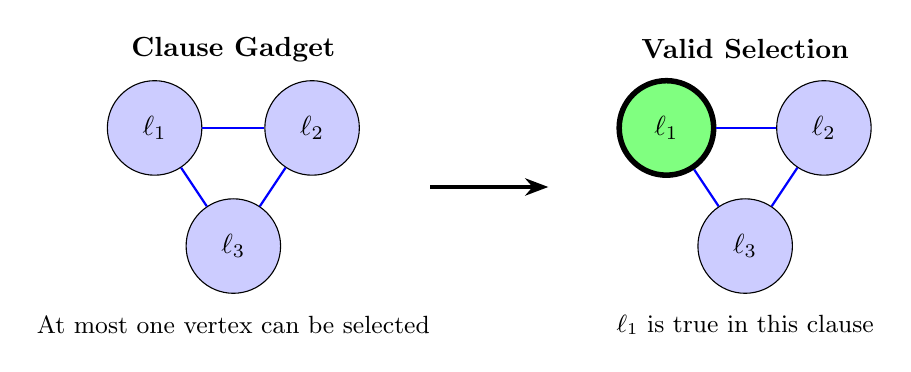
\begin{tikzpicture}[
    vertex/.style={circle, draw, fill=blue!20, minimum size=12mm, inner sep=1pt},
    selected/.style={circle, draw, fill=green!50, minimum size=12mm, inner sep=1pt, line width=2pt},
    clause_edge/.style={thick, blue},
    conflict_edge/.style={thick, red, dashed},
    scale=1.0
]
    % Single clause gadget illustration
    \node[vertex] (a) at (0, 0) {$\ell_1$};
    \node[vertex] (b) at (2, 0) {$\ell_2$};
    \node[vertex] (c) at (1, -1.5) {$\ell_3$};

    \draw[clause_edge] (a) -- (b);
    \draw[clause_edge] (b) -- (c);
    \draw[clause_edge] (c) -- (a);

    \node at (1, 1) {\textbf{Clause Gadget}};
    \node at (1, -2.5) {\small At most one vertex can be selected};

    % Arrow
    \draw[-{Stealth}, very thick] (3.5, -0.75) -- (5, -0.75);

    % Selected version
    \node[selected] (a2) at (6.5, 0) {$\ell_1$};
    \node[vertex] (b2) at (8.5, 0) {$\ell_2$};
    \node[vertex] (c2) at (7.5, -1.5) {$\ell_3$};

    \draw[clause_edge] (a2) -- (b2);
    \draw[clause_edge] (b2) -- (c2);
    \draw[clause_edge] (c2) -- (a2);

    \node at (7.5, 1) {\textbf{Valid Selection}};
    \node at (7.5, -2.5) {\small $\ell_1$ is true in this clause};
\end{tikzpicture}
\caption{The clause gadget enforces selecting at most one ``true'' literal per clause}
\end{figure}

\subsection{Proof of Correctness}

\begin{lemma}
$\phi$ is satisfiable if and only if $G_\phi$ has an independent set of size $m$.
\end{lemma}

\begin{proof}
$(\Rightarrow)$ Suppose $\phi$ is satisfiable with assignment $\alpha$. For each clause $C_j$, at least one literal is true under $\alpha$. Select one such true literal's vertex from each clause. This gives exactly $m$ vertices.

\textbf{Claim:} These vertices form an independent set.
\begin{itemize}
    \item No two selected vertices are from the same clause (we pick exactly one per clause), so no clause edges connect them.
    \item No two selected vertices have complementary labels (since $\alpha$ is consistent---it cannot set both $x_i$ and $\neg x_i$ to true), so no conflict edges connect them.
\end{itemize}

$(\Leftarrow)$ Suppose $G_\phi$ has an independent set $S$ of size $m$. Since each clause contributes a triangle and $S$ can contain at most one vertex from each triangle, and $|S| = m$, $S$ must contain exactly one vertex from each clause.

Define assignment $\alpha$: for each selected vertex labeled $\ell$:
\begin{itemize}
    \item If $\ell = x_i$, set $x_i = \texttt{true}$
    \item If $\ell = \neg x_i$, set $x_i = \texttt{false}$
\end{itemize}

\textbf{Claim:} $\alpha$ is well-defined and satisfies $\phi$.
\begin{itemize}
    \item Well-defined: If $S$ contained both $x_i$ and $\neg x_i$, they would be connected by a conflict edge, contradicting independence.
    \item Satisfies $\phi$: Each clause has a selected vertex, whose label is a true literal under $\alpha$.
\end{itemize}
\end{proof}

\section{Complexity Analysis}

\begin{theorem}
The reduction from Circuit SAT to Maximum Independent Set runs in polynomial time.
\end{theorem}

\begin{proof}
\textbf{Step 1 (Tseytin):}
\begin{itemize}
    \item Each gate produces $O(1)$ clauses with $O(1)$ literals
    \item Total: $O(|C|)$ clauses where $|C|$ is the circuit size
\end{itemize}

\textbf{Step 2 (3-SAT to MIS):}
\begin{itemize}
    \item $3m$ vertices (3 per clause)
    \item $O(m^2)$ edges (triangles plus conflict edges)
    \item Construction time: $O(m^2)$
\end{itemize}

Combined: $O(|C|^2)$ total time.
\end{proof}

\section{Complete Example}

Consider the circuit and formula from our running example. Here is the complete reduction visualized:

\begin{figure}[h]
\centering
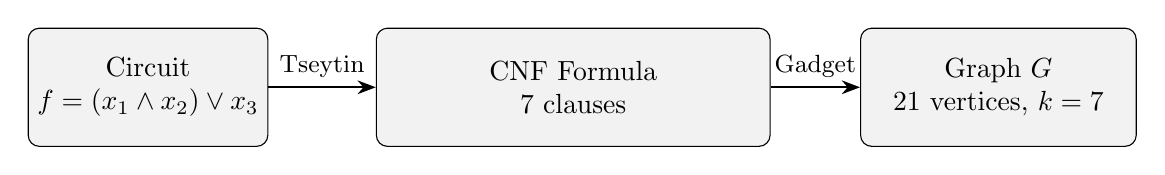
\begin{tikzpicture}[
    box/.style={rectangle, draw, rounded corners, minimum width=3cm, minimum height=1.5cm, align=center, fill=gray!10},
    arrow/.style={-{Stealth}, thick},
    scale=0.9
]
    % Circuit
    \node[box] (circuit) at (0, 0) {Circuit\\$f = (x_1 \land x_2) \lor x_3$};

    % CNF
    \node[box, minimum width=5cm] (cnf) at (6, 0) {CNF Formula\\7 clauses};

    % Graph
    \node[box, minimum width=3.5cm] (graph) at (12, 0) {Graph $G$\\21 vertices, $k=7$};

    \draw[arrow] (circuit) -- (cnf) node[midway, above] {\small Tseytin};
    \draw[arrow] (cnf) -- (graph) node[midway, above] {\small Gadget};
\end{tikzpicture}
\end{figure}

\section{Summary}

\begin{figure}[h]
\centering
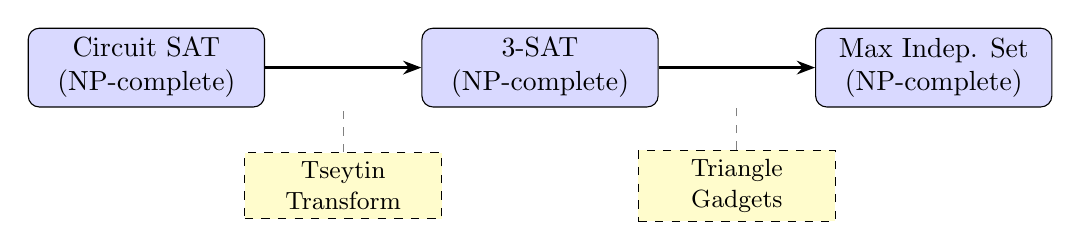
\begin{tikzpicture}[
    problem/.style={rectangle, draw, rounded corners, fill=blue!15, minimum width=3cm, minimum height=1cm, align=center},
    technique/.style={rectangle, draw, dashed, fill=yellow!20, minimum width=2.5cm, minimum height=0.8cm, align=center, font=\small},
    arrow/.style={-{Stealth}, thick}
]
    \node[problem] (csat) at (0, 0) {Circuit SAT\\(NP-complete)};
    \node[problem] (3sat) at (5, 0) {3-SAT\\(NP-complete)};
    \node[problem] (mis) at (10, 0) {Max Indep. Set\\(NP-complete)};

    \node[technique] (t1) at (2.5, -1.5) {Tseytin\\Transform};
    \node[technique] (t2) at (7.5, -1.5) {Triangle\\Gadgets};

    \draw[arrow] (csat) -- (3sat);
    \draw[arrow] (3sat) -- (mis);

    \draw[dashed, gray] (t1) -- (2.5, -0.5);
    \draw[dashed, gray] (t2) -- (7.5, -0.5);
\end{tikzpicture}
\caption{Summary of the reduction chain}
\end{figure}

\noindent\textbf{Key Points:}
\begin{enumerate}
    \item Circuit SAT captures all of NP (Cook-Levin theorem)
    \item Tseytin transformation: each gate $\to$ small CNF, linear blowup
    \item 3-SAT to MIS: clause triangles + conflict edges
    \item Both reductions are polynomial-time
    \item Therefore, Maximum Independent Set is NP-complete
\end{enumerate}

\section*{References}
\begin{enumerate}
    \item Tseytin, G. S. (1983). On the complexity of derivation in propositional calculus.
    \item Karp, R. M. (1972). Reducibility among combinatorial problems.
    \item Sipser, M. (2012). Introduction to the Theory of Computation. Cengage Learning.
\end{enumerate}

\end{document}
